\documentclass[herrin-thesis.tex]{subfiles}
\begin{document}

\chapter{The EXO-200 Detector}
\label{ch:detector}

\section{Creating a Sensitive Detector}
\label{sec:detector_sensitivity}
The number of decays of a radioactive element in a given period of time follow a Poisson distribution, provided the half-life is much longer than the observation time. This is clearly the case for a double beta decay experiment. The expected signal in such a case is
\begin{equation}
N_{s} = \epsilon \frac{a M}{m_{a}} \frac{t \ln2}{T_{1/2}}
\label{eq:detector_N_expected}
\end{equation}
events, where  \(\epsilon\) is the efficiency for detection, \(a\) is the isotopic abundance, \(M\) is the total mass of the element, \(m_{a}\) is the mass of a single atom, \(t\) is the total observation time, and \(T_{1/2}\) is the half life.

If an experiment observes no decays, then it sets a lower limit on the half life substituting for \(N_s\) a number that corresponds to a desired confidence level for the Poisson distribution. The sensitivity to the half-life, then, goes like
\begin{equation}
S(T_{1/2}) \propto \epsilon t \frac{a M}{m_{a}}
\label{eq:detector_bgfree_sensitivity}
\end{equation}

Now suppose that an experiment has some number \(N_b\) of background events in the region of interest. As an approximation, assume that the rate of background events \(b\) (in units of counts per unit energy per unit exposure) is flat over an energy-based region of interest, whose width \(\Gamma\) increases with the detector resolution. The number of background events then increases with increasing exposure \(M t\), or  \(N_b \propto b M t \Gamma\). The confidence limit on \(N_s\) must take into account the Poisson counting uncertainty on \((N_s + N_b)\), which will be dominated by the uncertainty on \(N_b\) (denoted \(\Delta N_b\)), and so the sensitivity instead goes like
\begin{equation}
S(T_{1/2}) \propto t \epsilon \frac{a M}{m_{a}} \frac{1}{\Delta N_b} \approx t \epsilon \frac{a M}{m_{a}} \frac{1}{\sqrt{N_b}} \propto \epsilon \frac{a}{m_{a}} \sqrt{\frac{M t}{b \Gamma}}
\label{eq:detector_bg_sensitivity}
\end{equation}
where the approximation that the uncertainty \(\Delta N_b = \sqrt{N_b}\) is valid when \(N_b\) is large enough that Gaussian statistics apply. Poisson statistics on \(N_b\) create a transition between \cref{eq:detector_bgfree_sensitivity,eq:detector_bg_sensitivity}.

The design of a detector for a double beta decay experiment is guided by \cref{eq:detector_bgfree_sensitivity,eq:detector_bg_sensitivity}. It must be able to contain a large mass \(M\) of material highly-enriched in the isotope of interest (large \(a\)). It must also have a good energy resolution (small \(\Gamma\)) and be constructed to minimize backgrounds (small \(b\)). In a search for \zeronu{}, recalling \cref{eq:nu_zeronu_rate}, an experiment with large backgrounds will decrease the smallest  \(\langle m_{\nu} \rangle\) it is sensitive to as \(t^{-1/4}\), which is much slower than an experiment with small backgrounds, which goes more like \(t^{-1/2}\). EXO-200 is designed to meet these goals to achieve good sensitivity.

\section{Time Projection Chamber}
\begin{figure}[htbp]
\centering
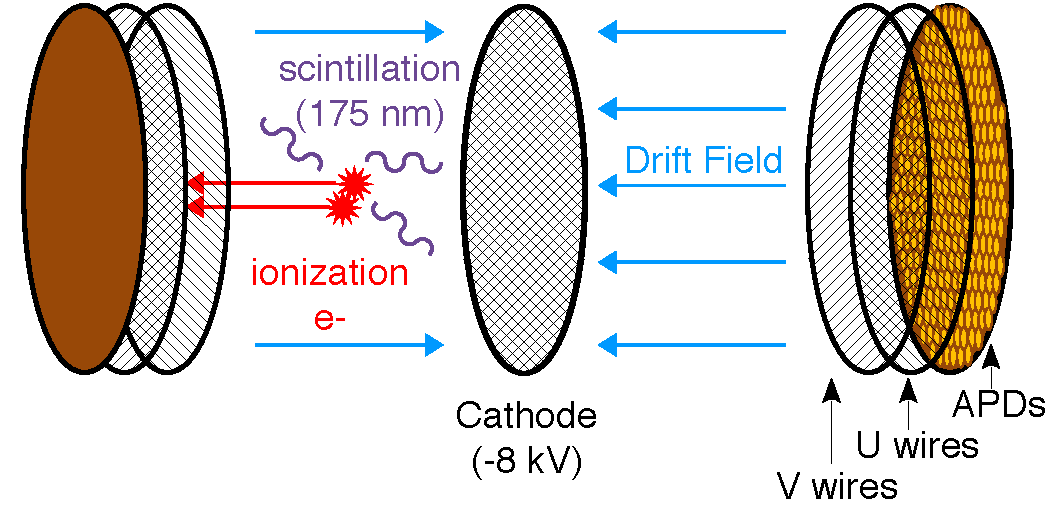
\includegraphics[width=0.75\textwidth]{./figures/detector_tpc_schematic.pdf}
\caption[A conceptual drawing of EXO-200]{The concept for EXO-200. The TPC is divided into two identical halves by a cathode. When energy is deposited in the liquid xenon, it creates both scintillation light and ionization. APDs behind the anode wire planes collect the scintillation signal. Ionization drifts to the anode and is read out on two crossed wire planes.}
\label{fig:detector_tpc_cartoon}
\end{figure}
The EXO-200 detector uses liquid xenon as both the source and the detector of double beta decays. It takes the form of a Time Projection Chamber (TPC) that collects both the ionization and scintillation signals so they can be combined to improve energy resolution as discussed in \cref{ch:liquidxe}. The TPC also collects information about event topology, which is useful for background rejection. \Cref{fig:detector_tpc_cartoon} illustrates the TPC concept.

\subsection{Scintillation Readout}

The scintillation light is collected by Large Area Avalanche PhotoDiodes (LAAPDs, or APDs). APDs can be manufactured with significantly lower radioactivity than traditional photomultiplier tubes. They operate well at cryogenic temperatures, and have a higher quantum efficiency than PMTs at \SI{178}{\nm}. However, APDs do suffer from increased noise and reduced gain compared to PMTs, but this is less of a concern at cryogenic temperatures and for the relatively high energies associated with double beta decay.

The 468 APDs are housed in two identical platters on either end of the TPC. The APDs are electrically connected to the platters, which provide \about~\SI{1.4}{\kV} bias. The platters are plated with \ce{Al} and \ce{MgF2} for improved reflectivity. PTFE tiles line the walls of the TPC and reflect light to improve the collection efficiency. One device is missing from each platter in order to make room for a diffuser that can deliver light from an external laser through an optical fiber for calibration purposes.

The APDs are electrically grouped together in gangs of 5 to 7. A phosphor bronze ``spider'' provides a common electrical connection to a gang, and mechanically holds them in the platter. Individual APDs vary significantly in the voltage needed to achieve a desired product of quantum efficiency and gain, and so the gangs are chosen in order to match electrically-similar devices \cite{Neilson:2009fk}. A trim voltage is then applied so that all gangs have similar performance.

\subsection{Ionization Readout}

\begin{figure}[htbp]
\centering
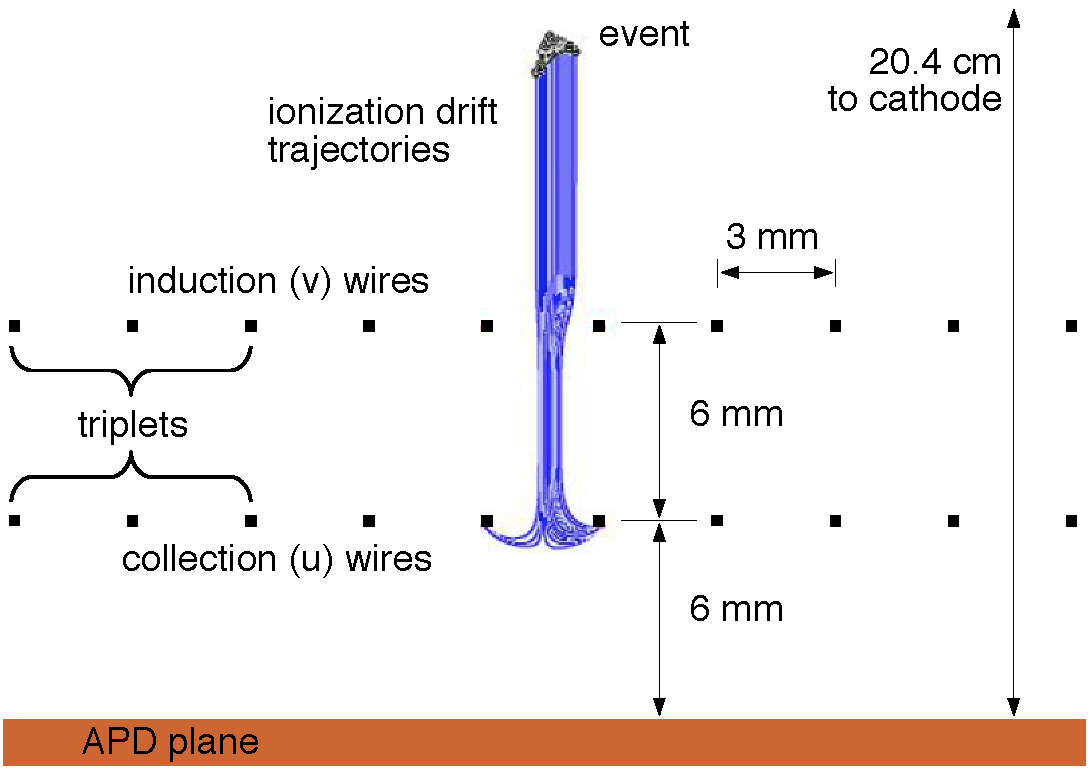
\includegraphics[width=0.6\textwidth]{./figures/detector_wire_geometry.pdf}
\caption[Geometry of the ionization readout wire planes]{The geometry of the ionization readout. An ionization cloud drifts past the \(v\) wires, inducing a signal in them. The cloud is then collected on the \(u\) wires. For simplicity, the wires are shown collinear here. In reality, they are angled \ang{60} from each other.}
\label{fig:detector_wire_geometry}
\end{figure}

A central cathode divides EXO-200 into two drift regions. This cathode creates a drift field that drifts ionization electrons to the anodes at either end of the TPC. The anodes consist of two crossed wire planes, angled \ang{60} to each other. The plane farther from the cathode, denoted \(u\), is held at virtual ground and collects the ionization. The plane closer to the cathode is denoted \(v\) and is biased to be fully transparent to drifting ionization. The \(v\) wire plane shields the \(u\) wire plane from induction effects. The induced signal on the \(v\) wires also provides a transverse coordinate. This, along with knowledge of which \(u\) wire collected the charge, provides a location for the event in the transverse plane. It is possible to reject backgrounds by using the multiplicity of signals (see \cref{sec:data_topology}) and location information to determine a fiducial volume (see \cref{sec:analysis_fiducial_volume}).

Each wire plane consists of 114 wires, spaced \SI{3}{\mm} apart. These wires were formed as triplets by photoetching sheets of phosphor bronze. This gives 38 electrical readouts per plane. Each wire plane is 95.8\% transparent to normally incident scintillation light. The cathode is also formed from two pieces of etched phosphor bronze and is 90\% transparent to normally incident light.

The wire planes are spaced \SI{6}{\mm} apart, and the collection plane is \SI{6}{\mm} from the face of the the platter that holds the APDs. The cathode, biased to \SI{-8}{\kV}, is \SI{19.2}{\cm} from the induction wire plane. The anode, cathode and cylindrical field shaping rings along the sides of the drift region create a \SI{374}{\V\per\cm} field in the main drift region. A chain of resistors divides the voltage along the 10 field shaping rings in each drift region so that the drift field is uniform. Charge in this region drifts at \SI{1.71}{\mm\per\micro\s}. The field is stronger between the \(u\) and \(v\) wires, and charge drifts about \SI{2.2}{\mm\per\micro\s} in this region.

\subsection{Construction}

\begin{figure}[htbp]
\centering
\begin{subfigure}[c]{0.42\linewidth}
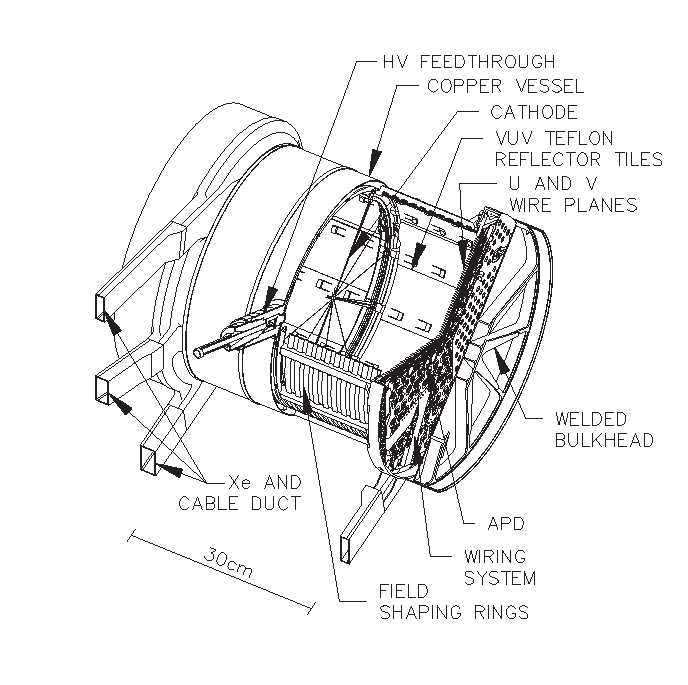
\includegraphics[width=\textwidth]{./photos/detector_TPC.pdf}
\end{subfigure}\hfill%
\begin{subfigure}[c]{0.54\linewidth}
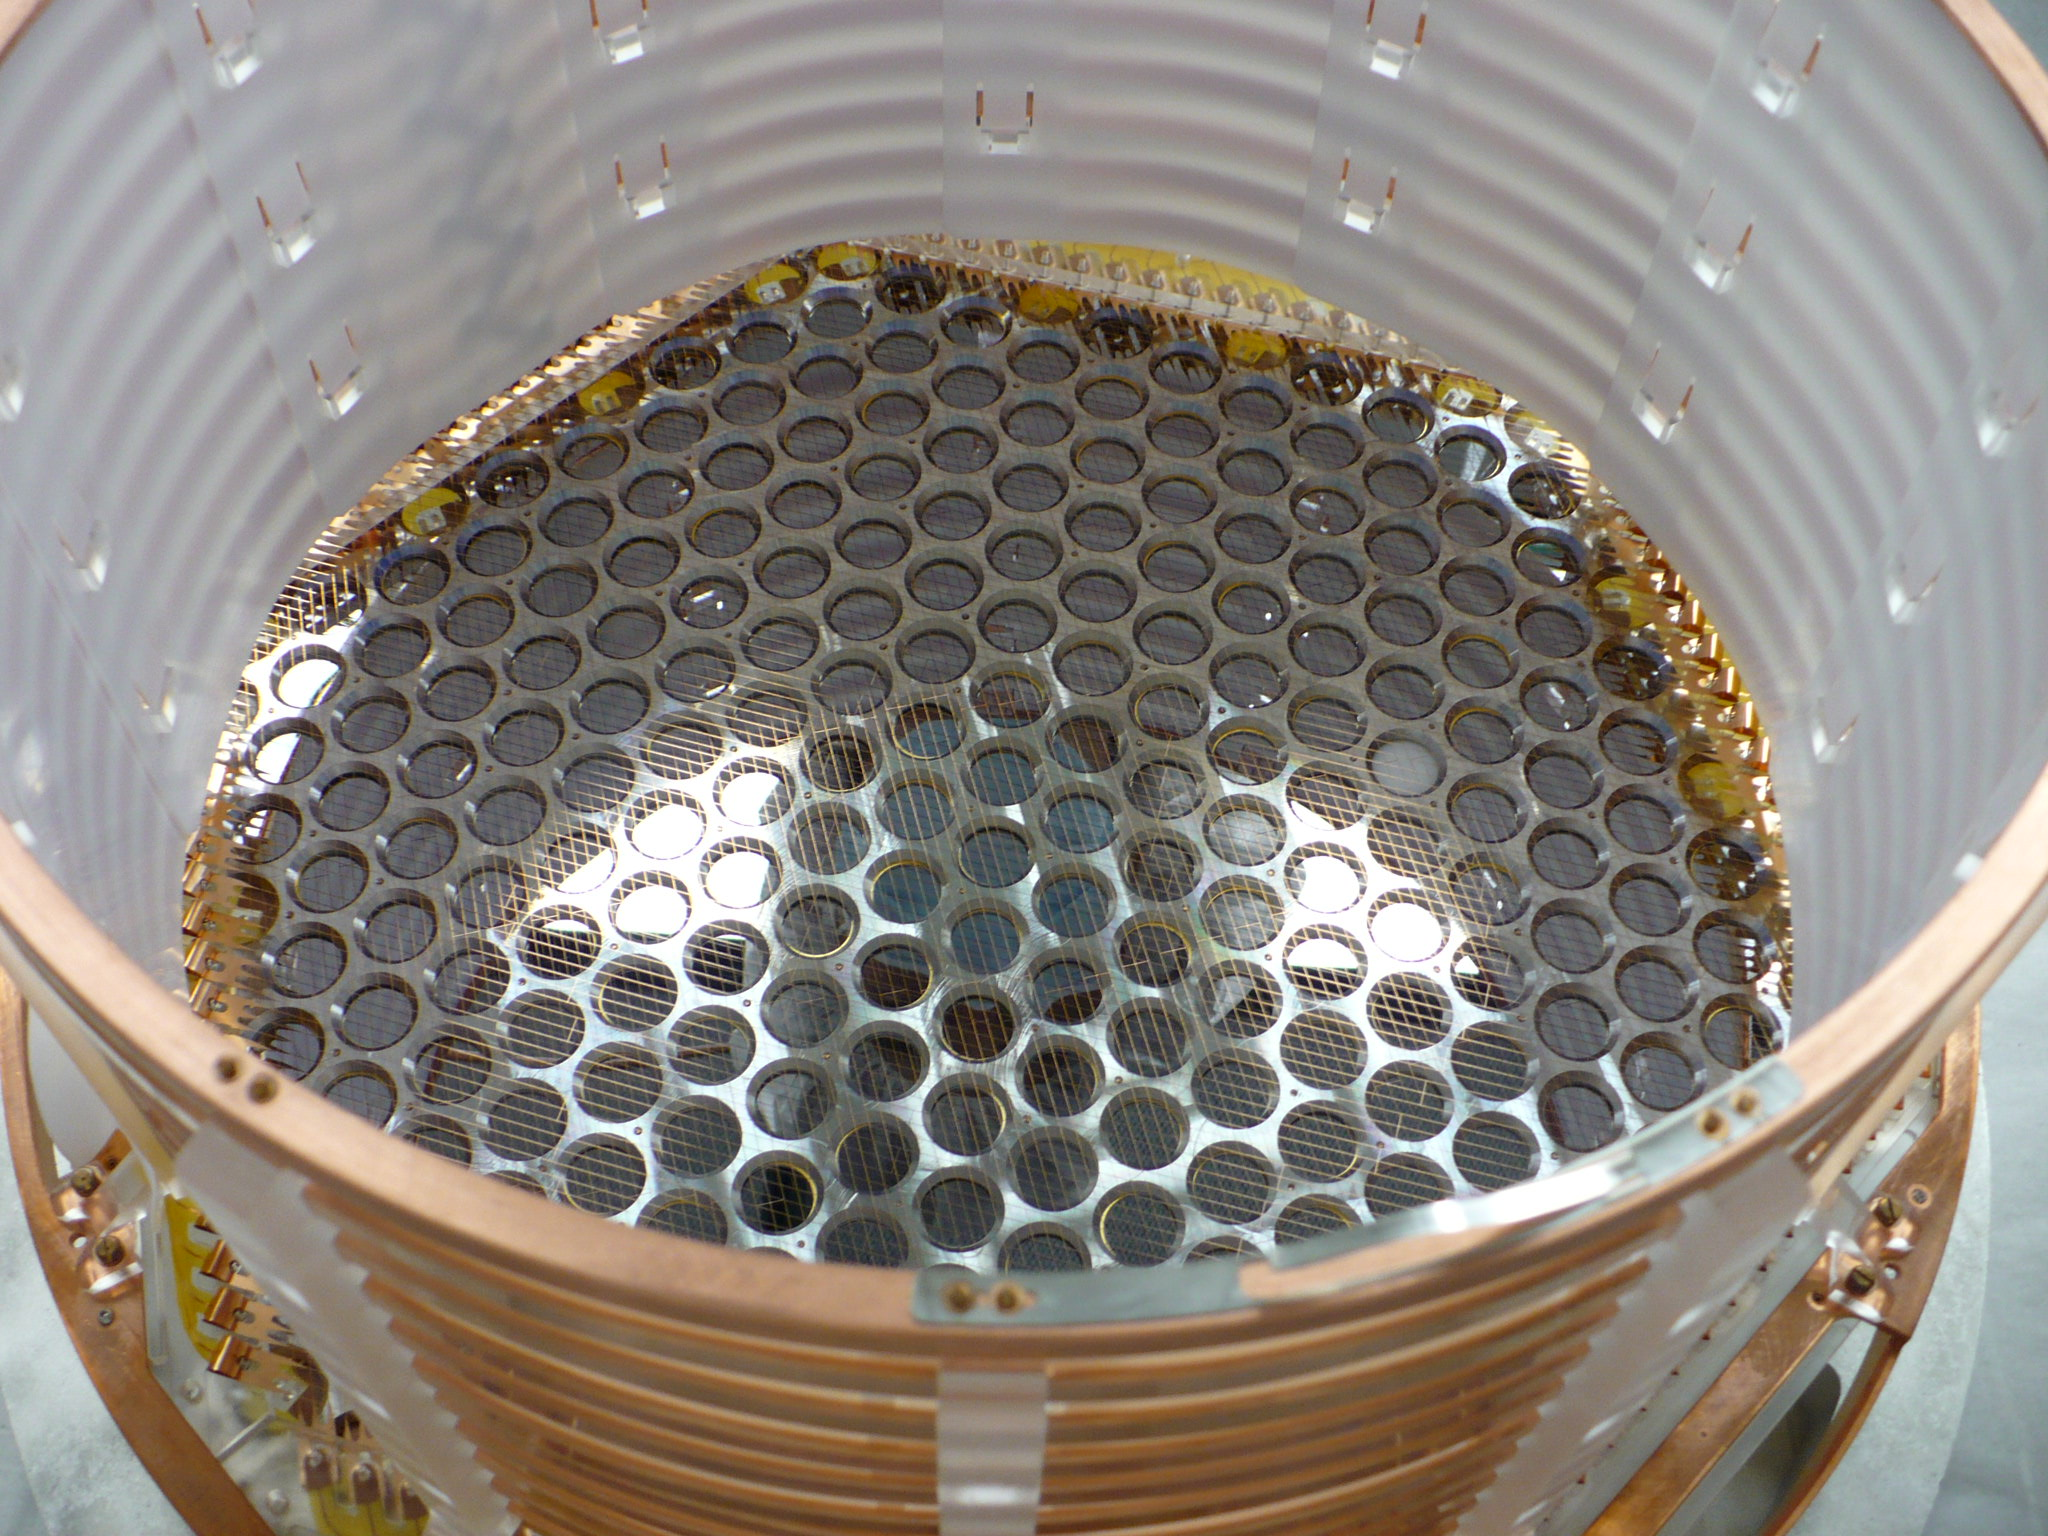
\includegraphics[width=\textwidth]{./photos/detector_half.jpg}
\end{subfigure}\hfill%
\caption[The EXO-200 detector]{On the left, a cutaway view of the EXO-200 detector and liquid xenon vessel. On the right is a photo of EXO-200 under construction. The circular APDs are visible in their platter and the flex cables can be seen around the edges. The anode wire planes are above the APD plane and cross each other at \ang{60}. PTFE tiles line the inside of the field-shaping rings. The cathode grid has not been installed in this photo, but would be at the top.}
\label{fig:detector_TPC_vessel}
\end{figure}

EXO-200 is made out of low-radioactivity copper, and was constructed under a modest concrete overburden to limit cosmogenic activation. The walls are only \SI{1.37}{\mm} thick to further reduce backgrounds due to radioactivity in the copper. All materials used in and around the detector have been thoroughly screened for radioactivity \cite{Leonard:2008uq}.

The electrical cables for the anode wires and the APDs reach the detector through six \about{}\SI{1}{\m} legs, which also support the detector horizontally from the cryostat door. Long cables allow the TPC to be shielded from any radioactivity in the electronics, at the expense of some electronic noise. These legs also allow liquid xenon to circulate through the detector. The high voltage reaches the cathode through a separate connection, located in the middle of the cylinder.

\section{Calibration}
\label{sec:detector_calibration}

\begin{figure}[htbp]
\centering
\begin{subfigure}[c]{0.33\linewidth}
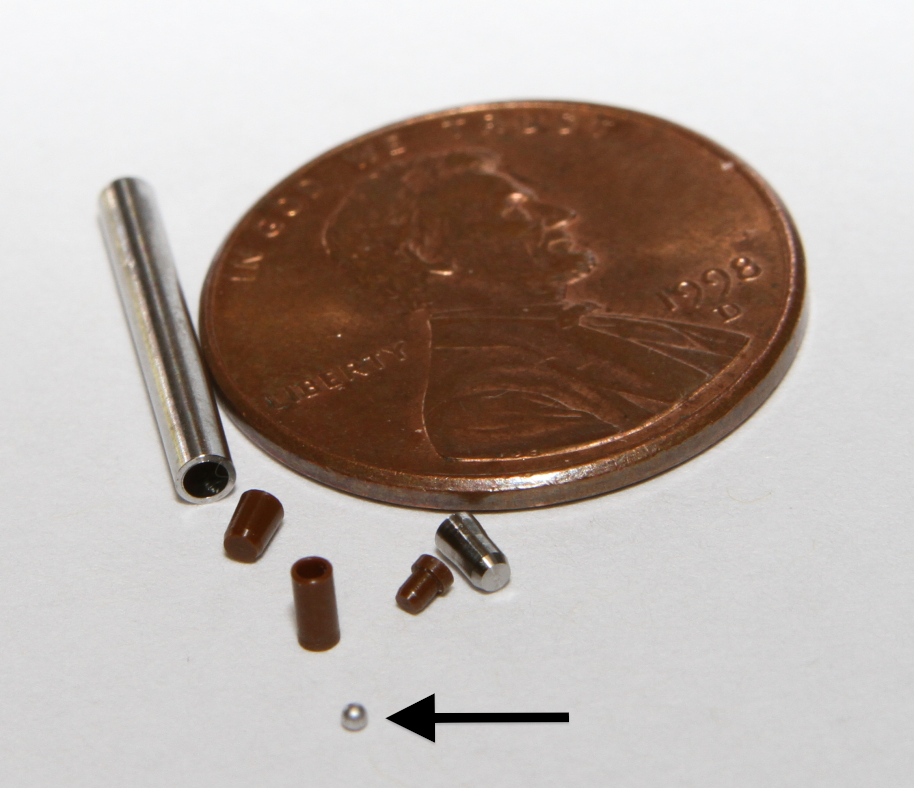
\includegraphics[width=\textwidth]{./photos/source_capsule_annotated.png}
\end{subfigure}\hspace{0.05\linewidth}\hfill%
\begin{subfigure}[c]{0.60\linewidth}
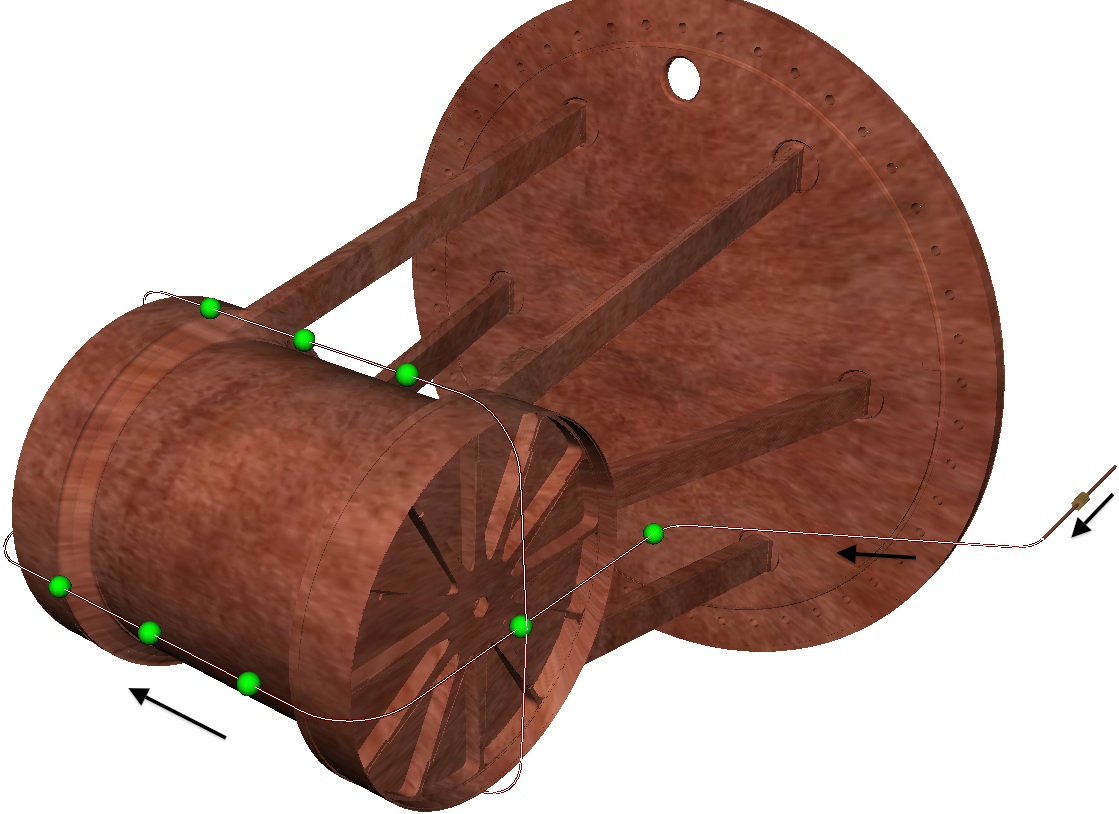
\includegraphics[width=\textwidth]{./photos/calibration_tubing_annotated.png}
\end{subfigure}
\caption[The calibration system]{To calibrate the detector, a tiny source capsule (left) containing a radioisotope housed in the small sphere indicated by the arrow can be pushed with a cable through a guide tube system to many positions just outside the detector (right).}
\label{fig:detector_calibration}
\end{figure}

Routine calibrations help monitor the performance and characterize the energy response of EXO-200. A guide tube system runs just outside the TPC, providing access to both anodes and three positions around the circumference of the cathode. In a typical calibration run, a miniature radioactive source is pushed to one of these positions by a long cable. After enough time passes to accumulate sufficient calibration data, the source is retracted and normal physics operations resume.

Currently, EXO-200 is calibrated with three different isotopes. \isotope{137}{Cs} emits a \SI{662}{\keV} gamma ray when it decays. \isotope{60}{Co} decays emit both \SI{1173}{\keV} and \SI{1333}{\keV} gamma rays simultaneously. \isotope{228}{Th} eventually decays to \isotope{208}{Tl}, which emits a \SI{2615}{\keV} gamma ray when it decays. Typically, short (\SI{2}{hr}) \isotope{228}{Th} calibrations are taken a few times per week, chiefly to measure the electron lifetime (see \cref{ch:electronlifetime}) and to track any other time variation in the detector response. Several times per year, longer campaigns with the full suite of sources establish the energy scale of the detector (see \cref{sec:data_calibration}).

\section{Infrastructure}

\begin{figure}[htbp]
\centering
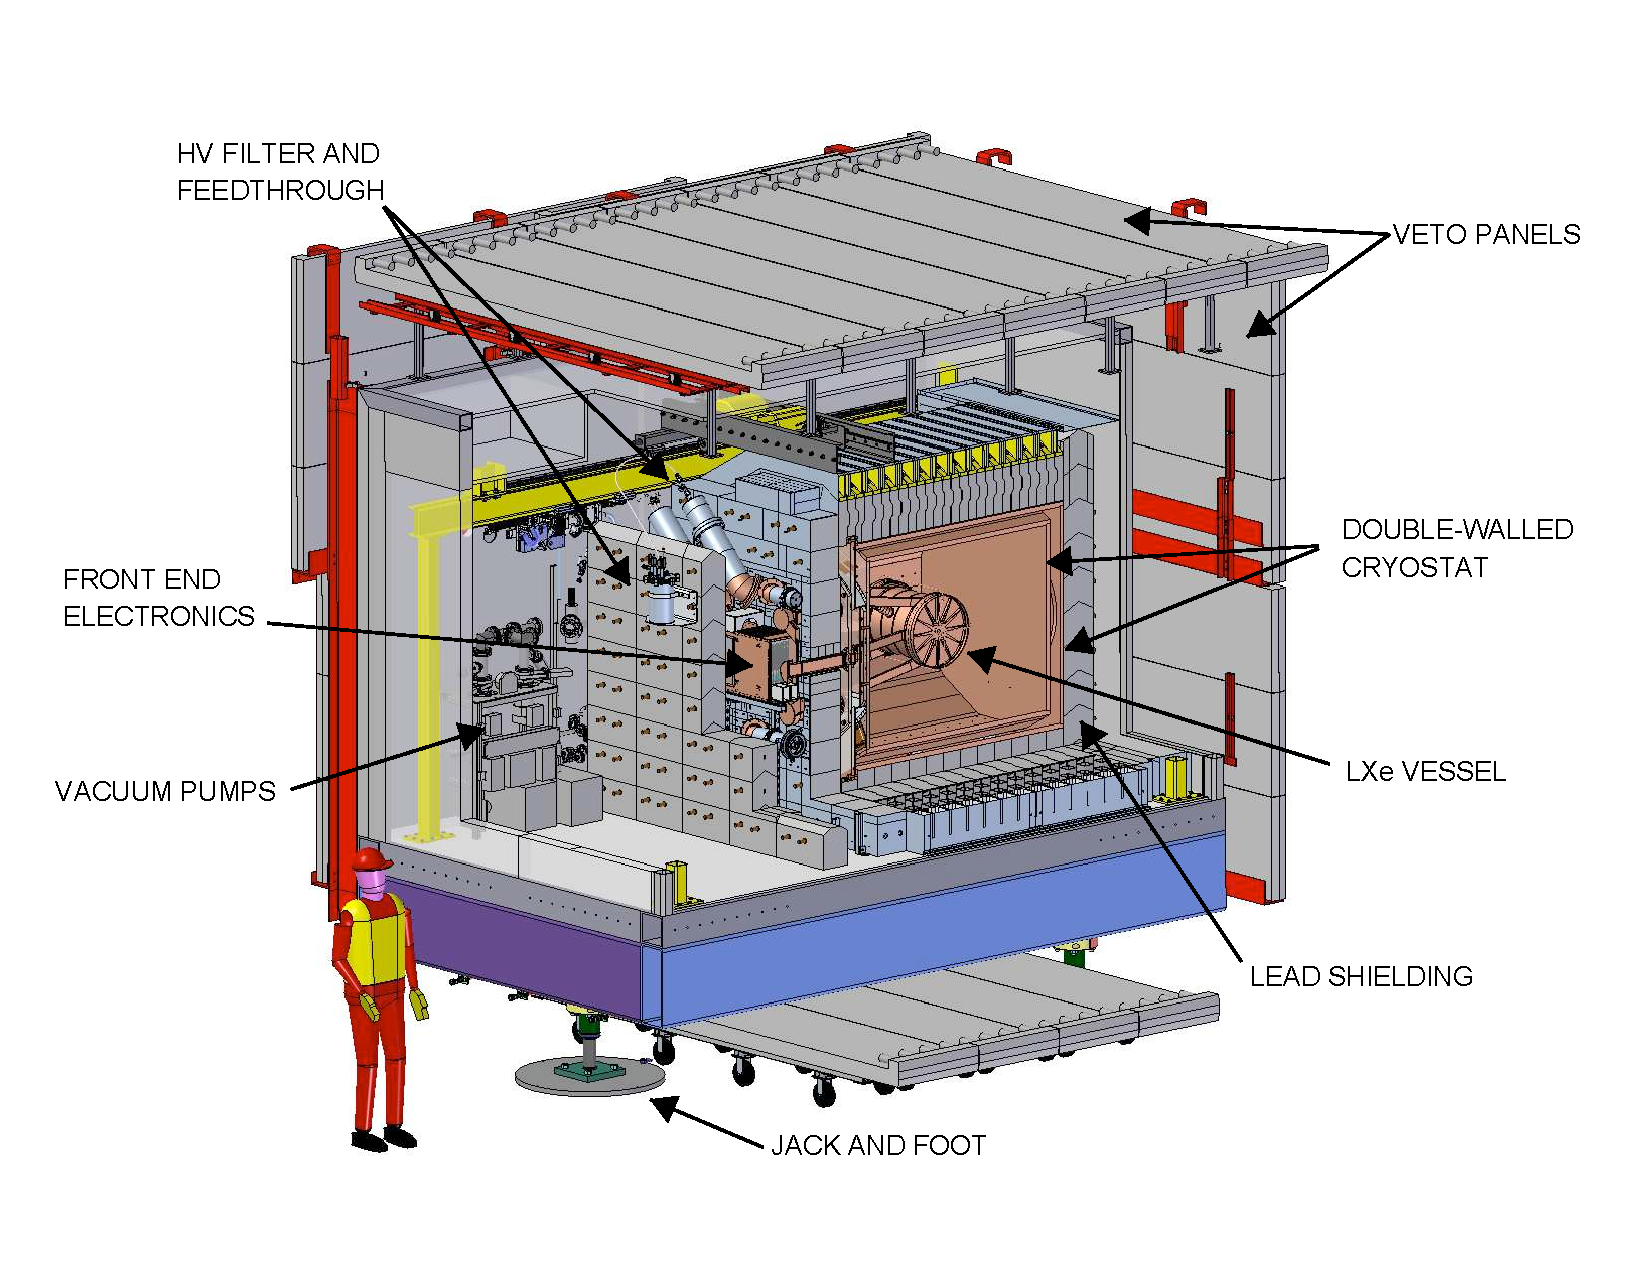
\includegraphics[width=1.0\textwidth]{./photos/detector_cleanroom.pdf}
\caption[Cutaway view of EXO-200 infrastructure]{A cutaway view of EXO-200 as installed at WIPP. The TPC vessel is surrounded by cold HFE. A cryostat insulates the HFE and liquid xenon. Lead surrounds the cryostat to shield from external radiation. All of this is located inside a clean room, which is surrounded with an active muon veto.}
\label{fig:detector_cleanroom}
\end{figure}

\subsection{Cryostat and Clean Rooms}
As shown in \cref{fig:detector_cleanroom}, the TPC vessel that contains the liquid xenon is housed inside a double-walled cryostat. The inner chamber is filled with HFE-7000 \cite{hfe7000} fluid that acts a thermal bath. The HFE fluid is radiologically clean and additionally provides some shielding from external \(\gamma\) radiation. The outer chamber is held at \(10^{-6}\)~\si{Torr} for insulation. The cryostat, made of copper low in radioactivity, is in turn shielded by \SI{25}{\cm} of lead on all sides. The front end electronics lie just outside this lead wall. On the front of the cryostat, a second \SI{25}{\cm} wall sits just outside the electronics. This second wall prevents external radiation from having line-of-site to the detector through the penetrations in the inner lead wall, used for xenon and electrical connections.

A class 1000 clean room houses the cryostat and its shielding in order to reduce trace radioactivity from dust being tracked in and introduced to the detector. This clean room also houses the xenon handling system, the cryogenic refrigerators used to chill the HFE, and other necessary infrastructure.

\subsection{Muon Veto}
While muons passing through the TPC can be readily identified (see \cref{ch:muons}), muons passing near the detector may still cause background events due to radiative processes and gamma rays from nuclear processes due to spallation neutrons. In order to reduce these backgrounds, the clean room housing the detector is surrounded by an active muon veto as shown in \cref{fig:detector_cleanroom}. Thirty-one plastic scintillator panels cover four sides of the clean room and detect \SI{96.0\pm0.5}{\%} of muons traversing the TPC.

\subsection{WIPP}

\begin{figure}[htbp]
\centering
\begin{subfigure}[c]{0.30\linewidth}
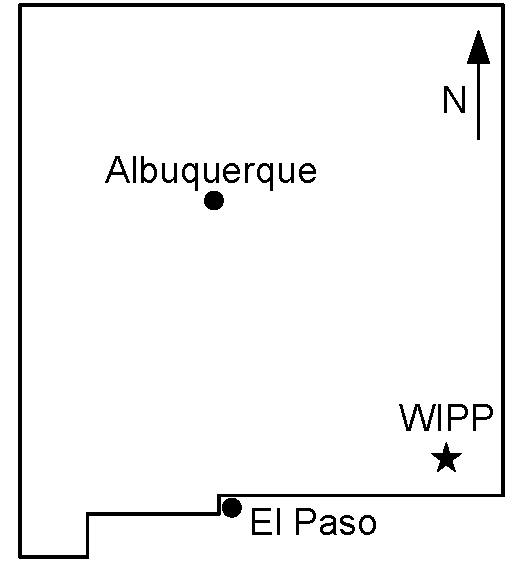
\includegraphics[width=\textwidth]{./figures/detector_wipp_map.pdf}
\end{subfigure}\hspace{0.05\linewidth}\hfill%
\begin{subfigure}[c]{0.60\linewidth}
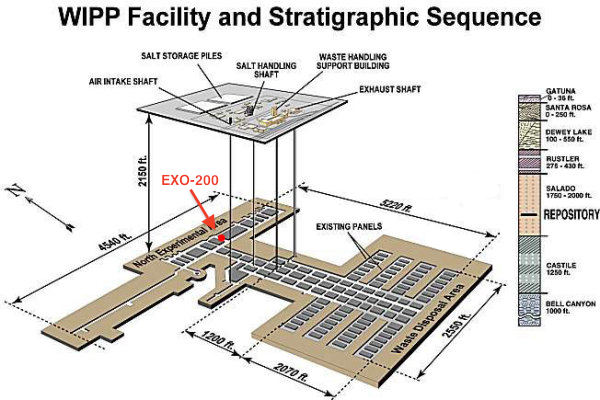
\includegraphics[width=\textwidth]{./photos/wipp_site_annotated.png}
\end{subfigure}
\caption[The WIPP site]{The left shows the location of the WIPP site on a map of New Mexico. The right shows a detailed view of the WIPP site. EXO-200 is located in the North Experimental Area, approximately \SI{655}{\m} underground. (Right image courtesy of the US Department of Energy.)}
\label{fig:detector_wipp}
\end{figure}

In order to attenuate the cosmic ray muons, EXO-200 is located \about{}\SI{655}{\m} underground at the Department of Energy's Waste Isolation Pilot Plant (WIPP) in southeastern New Mexico. WIPP is a salt mine, and its primary purpose is the permanent disposal of transuranic waste. The north end of the mine, far from and upwind of the waste, serves as a suitable site for low-background experiments.

The rock overburden provides \SI{1480}{\hecto\g\per\square\cm} shielding from cosmic rays (see \cref{ch:muons}), and the salt walls are naturally low in radionuclides. Direct counting finds a contamination of \SI[per-mode=symbol]{27\pm2d-9}{\g\per\g} of \isotope{238}{U}, \SI[per-mode=symbol]{66\pm2d-9}{\g\per\g} of \isotope{232}{Th}, and \SI[per-mode=symbol]{124\pm2d-9}{\g\per\g} of \isotope{40}{K} \cite{Auger:2012dq}. Little radon emanates from the walls, such that the radon concentration in the air is \SI{7}{\Bq\per\cubic\meter}, similar to that found at the surface.

\section{Xenon and Recirculation}
\label{sec:detector_xe_recirculation}

\begin{figure}[htbp]
\centering
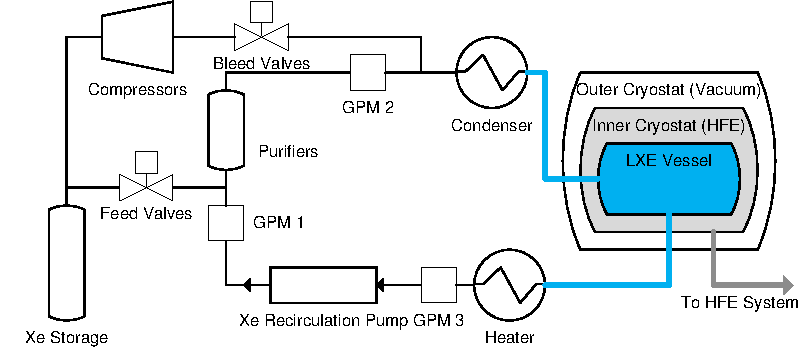
\includegraphics[width=0.9\textwidth]{./figures/detector_simplified_xe.pdf}
\caption[The EXO-200 xenon recirculation system]{A simplified schematic of the EXO-200 xenon recirculation system. A heater vaporizes xenon returning from the TPC. A gas-phase pump recirculates xenon through purifiers. The xenon is condensed and then returns to the TPC. Gas purity monitors (GPMs) look for changes in the electron lifetime of the circulating xenon. The TPC vessel must track the HFE pressure closely. A sophisticated slow controls system controls valves to feed and bleed xenon as needed from storage bottles. Compressors allow the xenon to be placed back into the bottles when bleeding xenon.}
\label{fig:detector_simplified_xe}
\end{figure}

As the name suggests, EXO-200 makes use of \SI{200}{\kg} of xenon enriched to 80.6\% in \xenon{136}. Of the remaining fraction of the xenon, isotope 134 comprises 19.1\%, and lighter natural isotopes are present in trace amounts. Roughly \SI{175}{\kg} of xenon fills the \SI{58}{\l} vessel, with \SI{110}{\kg} of that in the active region bounded by the anode wires and PTFE reflectors. The remaining xenon is in the recirculation and storage system.

The HFE is cooled to \SI{168}{\K} by cryogenic refrigerators through heat exchangers in the cryostat. Because the TPC vessel has very thin walls, the pressure inside must closely match the pressure of the HFE surrounding it. To keep the xenon in the liquid phase, the HFE is held at \about{}\SI{140}{\kilo\Pa} absolute pressure. A sophisticated slow control system can feed xenon gas into the system or bleed it off as needed to match this pressure. The xenon plumbing consists of a high pressure side where gas is stored, and a low pressure recirculation loop. Compressors place gas back into the storage bottles when bleeding. Under normal operations, feeds and bleeds do not happen. Instead, xenon returns from the TPC and vaporizes in a heater. A gas-phase pump \cite{LePort:2011fk} recirculates the xenon through purifiers, after which the xenon is recondensed. This is shown in \cref{fig:detector_simplified_xe}. 

The purifiers are heated \ce{Zr} getters \cite{SAESgetters} that chemically remove electronegative impurities from the xenon so that ionization can drift in the TPC. Gas purity monitors \cite{Dobi:2011zr} measure the quality of the gas returning from the TPC to look for large quantities of impurities, which might indicate purifier failure or a leak. However, in normal operation, continuous recirculation leads to electron lifetimes of \(>\)~\SI{2}{\ms}, which must be measured with the TPC itself  (see \cref{ch:electronlifetime}).

\section{Summary}
As this chapter and the even more thorough description in \cite{Auger:2012dq} describe, EXO-200 has been designed to be a sensitive double beta decay experiment. A large sample of xenon enriched in isotope 136 provides good exposure to signal events. Low background materials have been used throughout the construction, and layers of shielding provide additional protection. The detector itself is located deep underground to protect from cosmogenic activity. The TPC design allows for further background rejection through position-based fiducialization and by identifying Compton scattering gamma rays. The ionization and scintillation signals are combined to yield good energy resolution. All of these ensure a low background rate near the double beta decay endpoint. This in turn means good sensitivity to the double beta decay half life, and that the sensitivity should scale more like \cref{eq:detector_bgfree_sensitivity} than \cref{eq:detector_bg_sensitivity}.

\end{document}
